\subsection{Bubble \& eat - Responsabile Acquisti}
\begin{figure}[H]
	\centering
	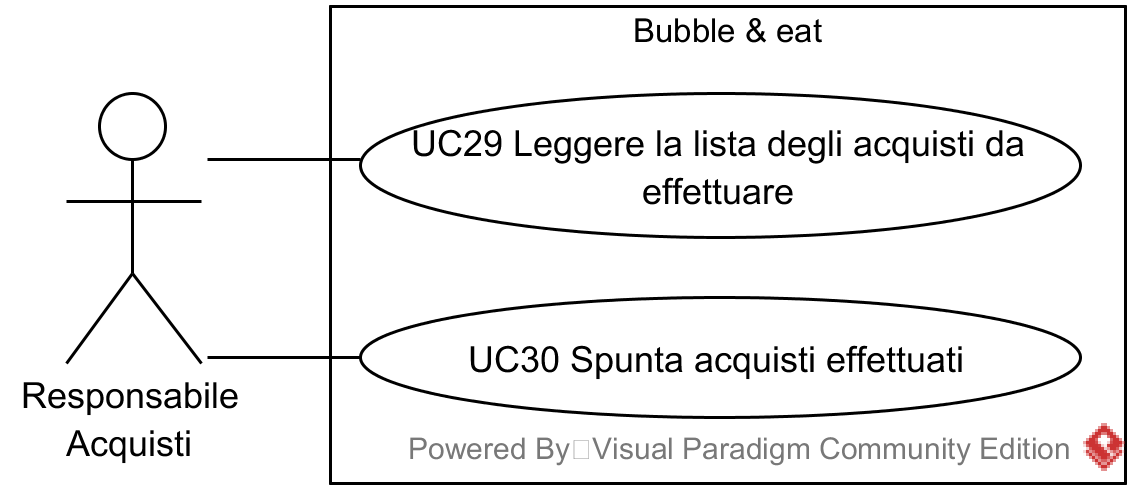
\includegraphics[width=15cm]{./Diagrammi_img/usecase/uc_bubble_responsabile_acquisti.png}
	\caption{Casi d'uso Bubble \& eat - Utente Responsabile Acquisti}
\end{figure}

\UC{Leggere la lista degli acquisti da effettuare}{UC3.7}

\begin{figure}[H]
	\centering
	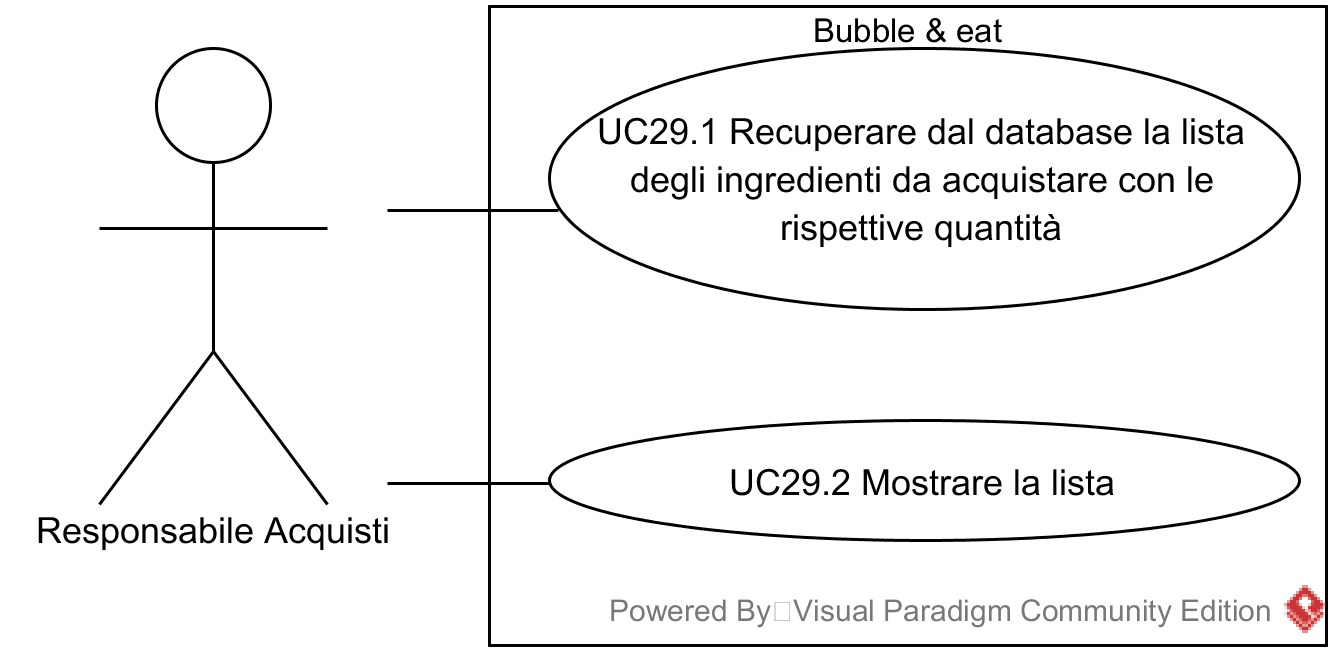
\includegraphics[width=15cm]{../../documenti/AnalisiDeiRequisiti/Diagrammi_img/usecase/uc3_7.png}
	\caption{\UCCaption{} Leggere la lista degli acquisti da effettuare}
\end{figure}

%\begin{figure}[H]
%	\centering
%	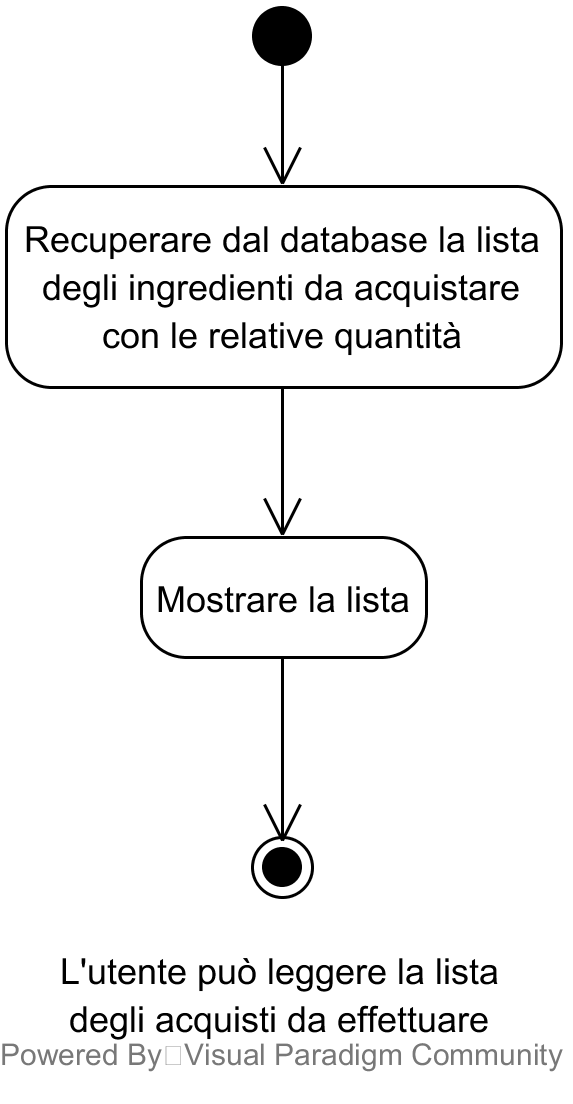
\includegraphics[height=10cm]{../../documenti/AnalisiDeiRequisiti/Diagrammi_img/attivita/uc_bubble_lista_acquisti.png}
%	\caption{Diagramma di attività - Leggere la lista degli acquisti da effettuare}
%\end{figure}

\begin{itemize}
	\item \textbf{Attori:}
	\\Responsabile Acquisti.
	\item \textbf{Scopo e descrizione:} 
	\\Lo scopo di questa funzionalità è permettere al Responsabile Acquisti di consultare la lista degli acquisti da effettuare.
	\item \textbf{Precondizioni:}
	\begin{itemize}
		\item Avere Rocket.Chat.
		\item Avere la bubble del ristorante selezionato.
		\item Avere accesso alla bubble con il ruolo di Responsabile Acquisti.
	\end{itemize}
	\item \textbf{Flusso principale degli eventi:}
	\begin{itemize}
		\item Il Responsabile Acquisti seleziona la parte corrispondente della bubble.
		\item Viene recuperata dal database la lista degli ingredienti \ref{UC3.7.1}.
		\item La lista viene mostrata all'utente \ref{UC3.7.2}.
	\end{itemize}
	\item \textbf{Post-condizione:}
	\\Il Responsabile Acquisti è a conoscenza dei prodotti da acquistare.
\end{itemize}

\UCF{Recuperare dal database la lista degli ingredienti da acquistare con le rispettive quantità}{UC3.7.1}

\begin{itemize}
	\item \textbf{Attori:}
	\\Responsabile Acquisti.
	\item \textbf{Scopo e descrizione:} 
	\\Lo scopo di questa funzionalità è di caricare all'interno della bubble la lista degli ingredienti da acquistare con le rispettive quantità.
	\item \textbf{Precondizioni:}
	\begin{itemize}
		\item Avere Rocket.Chat.
		\item Avere la bubble del ristorante selezionato.
		\item Avere accesso alla bubble con il ruolo di Responsabile Acquisti.
	\end{itemize}
	\item \textbf{Flusso principale degli eventi:}
	\\Il Responsabile Acquisti richiede di visualizzare la lista e la bubble la carica dal database.
	\item \textbf{Post-condizione:}
	\\La lista degli ingredienti è stata caricata all'interno della bubble.
\end{itemize}

\UCF{Mostrare la lista al Responsabile Acquisti}{UC3.7.2}

\begin{itemize}
	\item \textbf{Attori:}
	\\Responsabile Acquisti.
	\item \textbf{Scopo e descrizione:} 
	\\Lo scopo di questa funzionalità è rendere il Responsabile Acquisti conscio delle quantità e di cosa è incaricato di comprare.
	\item \textbf{Precondizioni:}
	\begin{itemize}
		\item Avere Rocket.Chat.
		\item Avere la bubble del ristorante selezionato.
		\item Avere accesso alla bubble con il ruolo di Responsabile Acquisti.
	\end{itemize}
	\item \textbf{Flusso principale degli eventi:}
	\\Il Responsabile Acquisti guarda la bubble interattiva.
	\item \textbf{Post-condizione:}
	\\Il Responsabile Acquisti è a conoscenza dei prodotti da acquistare.
\end{itemize}

\UC{Spunta acquisti effettuati}{UC3.8}

\begin{figure}[H]
	\centering
	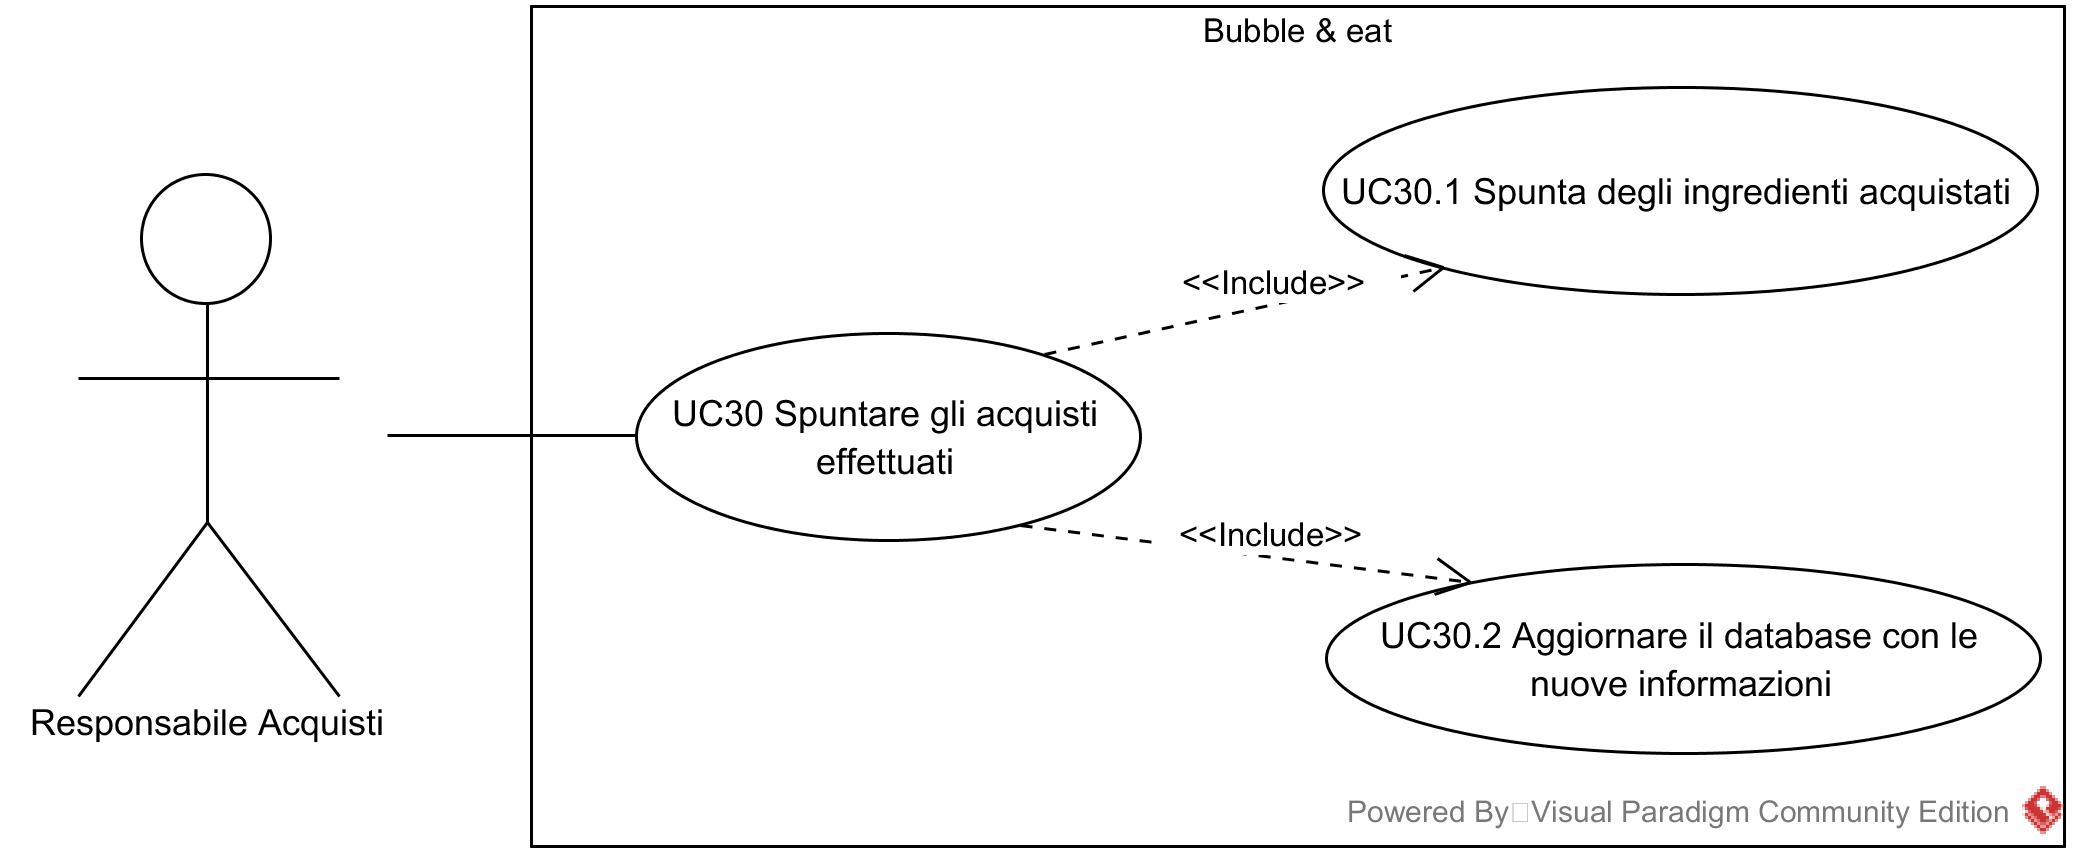
\includegraphics[width=15cm]{../../documenti/AnalisiDeiRequisiti/Diagrammi_img/usecase/uc3_8.png}
	\caption{\UCCaption{} Spunta acquisti effettuati}
\end{figure}

%\begin{figure}[H]
%	\centering
%	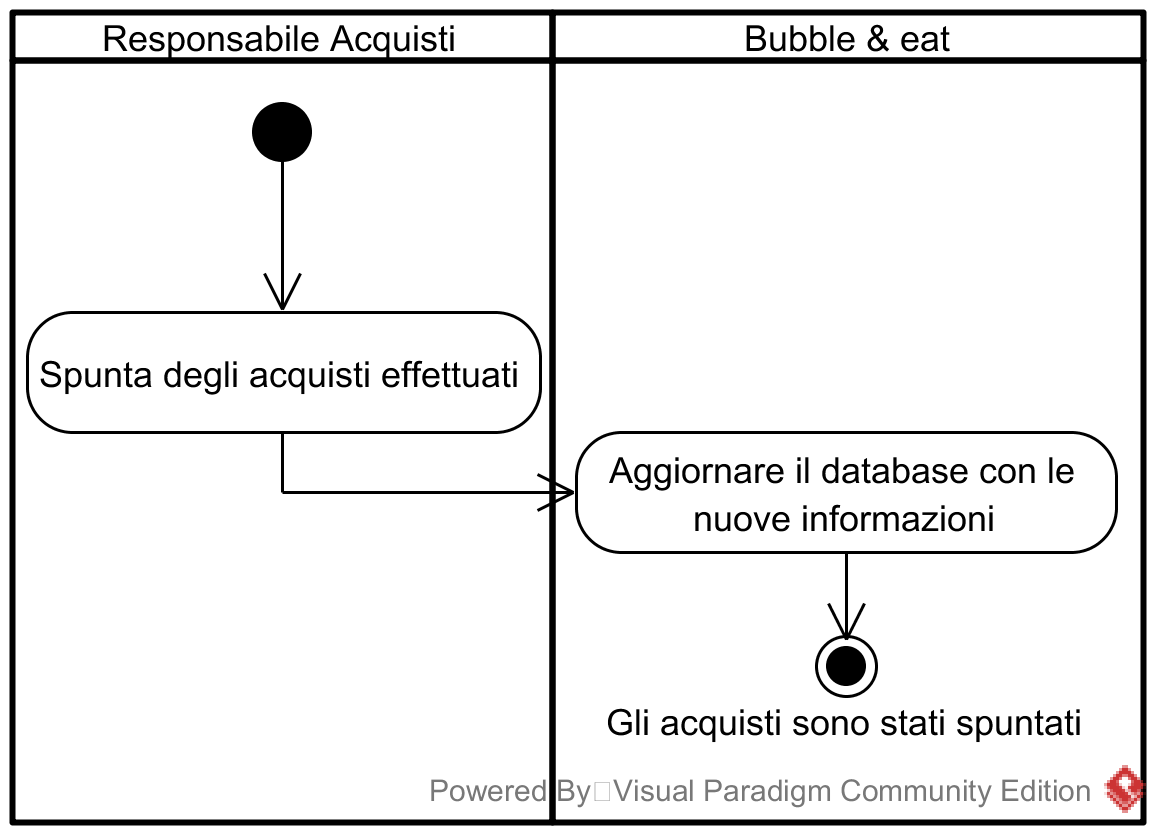
\includegraphics[height=10cm]{../../documenti/AnalisiDeiRequisiti/Diagrammi_img/attivita/uc_bubble_spunta_acquisti.png}
%	\caption{Diagramma di attività - Spunta acquisti effettuati}
%\end{figure}

\begin{itemize}
	\item \textbf{Attori:}
	\\Responsabile Acquisti.
	\item \textbf{Scopo e descrizione:} 
	\\Gli acquisti da effettuare presenti nella lista possono essere spuntati quando il Responsabile Acquisti ha acquisito un prodotto nella lista acquisti.
	\item \textbf{Precondizioni:}
	\begin{itemize}
		\item Avere Rocket.Chat.
		\item Avere la bubble del ristorante selezionato.
		\item Avere accesso alla bubble con il ruolo di Responsabile Acquisti.
		\item Visualizzare la lista degli acquisti da effettuare \ref{UC3.7.2}.
	\end{itemize}
	\item \textbf{Flusso principale degli eventi:}
	\\Il Responsabile Acquisti spunta una voce della lista.
	\item \textbf{Post-condizione:}
	\\La voce della lista acquisti è stata spuntata.
\end{itemize}

\UCF{Spunta degli ingredienti acquistati}{UC3.8.1}

\begin{itemize}
	\item \textbf{Attori:}
	\\Responsabile Acquisti.
	\item \textbf{Scopo e descrizione:} 
	\\Questa funzionalità permette al Responsabile Acquisti di segnalare i prodotti acquistati.
	\item \textbf{Precondizioni:}
	\begin{itemize}
		\item Avere Rocket.Chat.
		\item Avere la bubble del ristorante selezionato.
		\item Avere accesso alla bubble con il ruolo di Responsabile Acquisti.
		\item Visualizzare la lista degli acquisti da effettuare \ref{UC3.7.2}.
	\end{itemize}
	\item \textbf{Flusso principale degli eventi:}
	\\I dati vengono inseriti dal Responsabile Acquisti.
	\item \textbf{Post-condizione:}
	\\I dati sono pronti per essere aggiornati nel database.
\end{itemize}

\UCF{Aggiornare il database con le nuove informazioni}{UC3.8.2}

\begin{itemize}
	\item \textbf{Attori:}
	\\Responsabile Acquisti.
	\item \textbf{Scopo e descrizione:} 
	\\Lo scopo di questa funzionalità è quello di registrare all'interno del database i cambiamenti che sono avvenuti nelle quantità degli ingredienti, come conseguenza degli acquisti del Responsabile Acquisti.
	\item \textbf{Precondizioni:}
	\begin{itemize}
		\item Avere Rocket.Chat.
		\item Avere la bubble del ristorante selezionato.
		\item Avere accesso alla bubble con il ruolo di Responsabile Acquisti.
		\item Visualizzare la lista degli acquisti da effettuare \ref{UC3.7.2}.
		\item Il Responsabile Acquisti ha inserito i dati degli ingredienti acquistati.
	\end{itemize}
	\item \textbf{Flusso principale degli eventi:}
	\\Il Responsabile Acquisti ha inserito i dati degli ingredienti acquistati all'interno della bubble, la quale aggiorna il database.
	\item \textbf{Post-condizione:}
	\\Il database possiede le informazioni aggiornate sulla quantità degli ingredienti.
\end{itemize}